\documentclass[11pt, a4 paper]{article}
% Set target color model to RGB
\usepackage[inner=2.0cm,outer=2.0cm,top=2.5cm,bottom=2.5cm]{geometry}
\usepackage{setspace}
\usepackage[rgb]{xcolor}
\usepackage{verbatim}
\usepackage{subcaption}
\usepackage{amsgen,amsmath,amstext,amsbsy,amsopn,amssymb}
\usepackage{fancyhdr}
\usepackage[colorlinks=true, urlcolor=blue,  linkcolor=blue, citecolor=blue]{hyperref}
\usepackage[colorinlistoftodos]{todonotes}
\usepackage{rotating}
%\usetikzlibrary{through,backgrounds}
\hypersetup{%
pdfauthor={Ashudeep Singh},%
pdftitle={Homework},%
pdfkeywords={Tikz,latex,bootstrap,uncertaintes},%
pdfcreator={PDFLaTeX},%
pdfproducer={PDFLaTeX},%
}
%\usetikzlibrary{shadows}
% \usepackage[francais]{babel}
\usepackage{ctex}
\usepackage{booktabs}
\usepackage{fontspec}
\setmainfont{FandolSong}
\setmainfont[BoldFont=ArialBold.ttf,ItalicFont=ArialItalic.ttf]{Arial.ttf}
\newcommand{\ra}[1]{\renewcommand{\arraystretch}{#1}}

\newtheorem{thm}{Theorem}[section]
\newtheorem{prop}[thm]{Proposition}
\newtheorem{lem}[thm]{Lemma}
\newtheorem{cor}[thm]{Corollary}
\newtheorem{defn}[thm]{Definition}
\newtheorem{rem}[thm]{Remark}
\numberwithin{equation}{section}

\newcommand{\homework}[6]{
   \pagestyle{myheadings}
   \thispagestyle{plain}
   \newpage
   \setcounter{page}{1}
   \noindent
   \begin{center}
   \framebox{
      \vbox{\vspace{2mm}
    \hbox to 6.28in { {\bf Custom Intelligent Hardware Lab from Fudan University \hfill {\small (#2)}} }
       \vspace{6mm}
       \hbox to 6.28in { {\Large \hfill #1  \hfill} }
       \vspace{6mm}
       \hbox to 6.28in { {\it Principal Investigator: {\rm #3} \hfill Name: {\rm #5}, University: {\rm #6}} }
       %\hbox to 6.28in { {\it TA: #4  \hfill #6}}
      \vspace{2mm}}
   }
   \end{center}
   \markboth{2025 CiHLab -- #1}{2025 CiHLab -- #1}
   \vspace*{4mm}
}

\newcommand{\problem}[2]{~\\\fbox{\textbf{Problem #1}}\hfill (#2 points)\newline\newline}
\newcommand{\subproblem}[1]{~\newline\textbf{(#1)}}
\newcommand{\D}{\mathcal{D}}
\newcommand{\Hy}{\mathcal{H}}
\newcommand{\VS}{\textrm{VS}}
\newcommand{\solution}{~\newline\textbf{\textit{(Solution)}} }

\newcommand{\bbF}{\mathbb{F}}
\newcommand{\bbX}{\mathbb{X}}
\newcommand{\bI}{\mathbf{I}}
\newcommand{\bX}{\mathbf{X}}
\newcommand{\bY}{\mathbf{Y}}
\newcommand{\bepsilon}{\boldsymbol{\epsilon}}
\newcommand{\balpha}{\boldsymbol{\alpha}}
\newcommand{\bbeta}{\boldsymbol{\beta}}
\newcommand{\0}{\mathbf{0}}
\usepackage{enumitem}


\begin{document}

\homework{Pre-Summer-Camp Exam}{Due: 05/08/25}{Chixiao Chen}{}{Yutong Jia}{JiLin University}


\begin{itemize}
    \item This exam is open to textbooks and LLM AI tools. If you use LLM chatbots, please attach the initial AI generated contents, and briefly summary your own contribution. Do NOT discuss with other students.
    \item We care more about your ability to think critically and your knowledge acquisition beyond textbooks. Correctness is less of a concern.
    \item Please submit your response sheet in ONE PDF file and send it to Dr. Chen via: \url{cxchen2.uw@gmail.com} before 05/08/2025 11:59 pm. Please use "CiHLab-PreSCE-2025+YourName" as the mail title and PDF file name. 
    \item After your submission, you should receive an acknowledgment from me within three days. If not, please contact me again. 
    \item It is encouraged to use \LaTeX~to edit it, the source code of the assignment is available via: \\
    \url{https://www.overleaf.com/read/yddxwnmhhtzj#ea4de1}
    \item You can also answer the problems by opening and editing the exam PDF using Office/WPS WORD for easy editing. Also, you can print it out, handwrite your responses, and scan it with your cellphone.
    \item You can answer the assignment either in Chinese or English. 
    \item For Problem 3-6, you only need to complete \textbf{TWO} of them. If you solve more than 2 problems, only the highest two scores would be counted.
    
\end{itemize}
\newpage
\section{Summary Of My Answer}
感谢陈老师和Cihlab给我一个机会参与入组考核,我很荣幸能够借此机会与陈老师通过问题-答案的形式交流。除了问题1,2,7是必须完成的以外,选做题中我完成的是问题3和问题5。针对每一个问题的解答,我往往会按照问题分析-背景知识-问题解答-总结的步骤完成。接下来是我的解答部分,我没有完成的内容被从该文件中删除。

\problem{1: Hardware Description Language}{15}
Design a 4-bit synchronous counter with a synchronous reset input that resets the counter to zero. The counter wraps around on overflow (modulo 16).
The optimization target is to use as few gates as possible, and please approximate the gate count (in terms of 1-input inverters and D-Flip-Flops) of your design according to the HDL script.

Please write the HDL of the counter in either Verilog, SystemVerilog, or Chisel. 

\section{The Answer to Problem 1}
\subsection{Problem Analysis}
本问题中共包含两点要求:
\begin{enumerate}[nosep]
    \item 设计一个具有同步复位的4bit同步计数器,溢出时按对16取模进行循环;
    \item 尽可能优化它使用的门电路数量,以1输入反相器和D触发器数量为衡量标准。
\end{enumerate}
\subsection{Background Knowledge}
在完成这道题目之前,有几个关键的基础知识需要回顾一下。
\begin{itemize}
    \item \textbf{D-Filp-Flops:} D触发器是从JK触发器演变而来的一种常用触发器,对JK触发器取$J=\overline{K}=D$,则得到D触发器。它的特征方程如下:
    $$\begin{cases}&Q^n=J\overline{Q}^n+\overline{K}^nQ^n=D\overline{Q}^n+DQ^n\\&Q^{n+1}=D\end{cases}$$
    在本题的解答中,使用Vivado作为分析综合软件,其中包含多种D触发器,它们的区别如下所示:
    
    \begin{figure}[h]
    \centering
    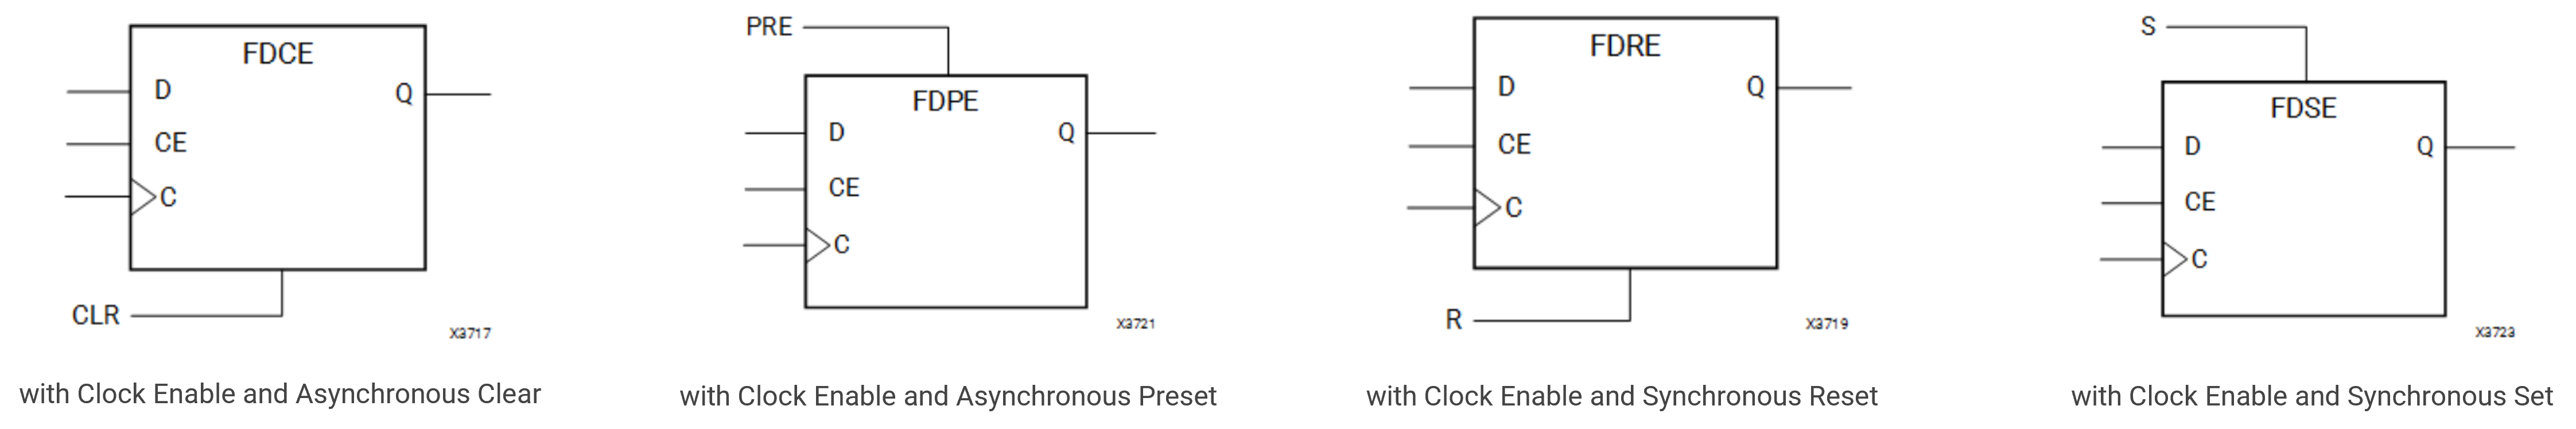
\includegraphics[width=1\linewidth]{image/Xilinx_D_Filp_Flop.png}
    \end{figure}
    工具将会根据代码自己决定使用的D触发器。根据本题的要求,实际使用的是FDRE,带有时钟使能和同步复位的D触发器。值得注意的是,它的复位信号被配置为高电平有效,因此如果使用低电平有效的复位信号将额外产生一个反向器。
    \item \textbf{Fatch \& Flip-Flop:} 锁存器和触发器都是数字电路中的基本储存单元,但锁存器由电平触发,往往出现在组合电路中,受到使能信号控制;触发器由边沿触发,出现在时序电路中,受到时钟信号控制;锁存器往往由于设计缺陷导致自动推断出锁存器,导致时序难以控制;触发器是时序逻辑中的正常实现方法。因此在设计中应当尽量避免出现锁存器,包括避免情况覆盖不完全的if-else等。
\end{itemize}
\subsection{Problem Solving}
\subsubsection{The Principle of The Synchronous Counter}
根据二进制加法运算规则可知,在一个多为二进制数末尾上加1时,若其中第i位一下各位皆为1时,第i位应改变状态(1变成0,0变成1),而最低为的状态在每次加1时都要改变。若使用D触发器进行实现,需要搭配加法器或LUT完成。使用D触发器设计的同步计数器原理图如下所示:
\begin{figure}[h]
    \centering
    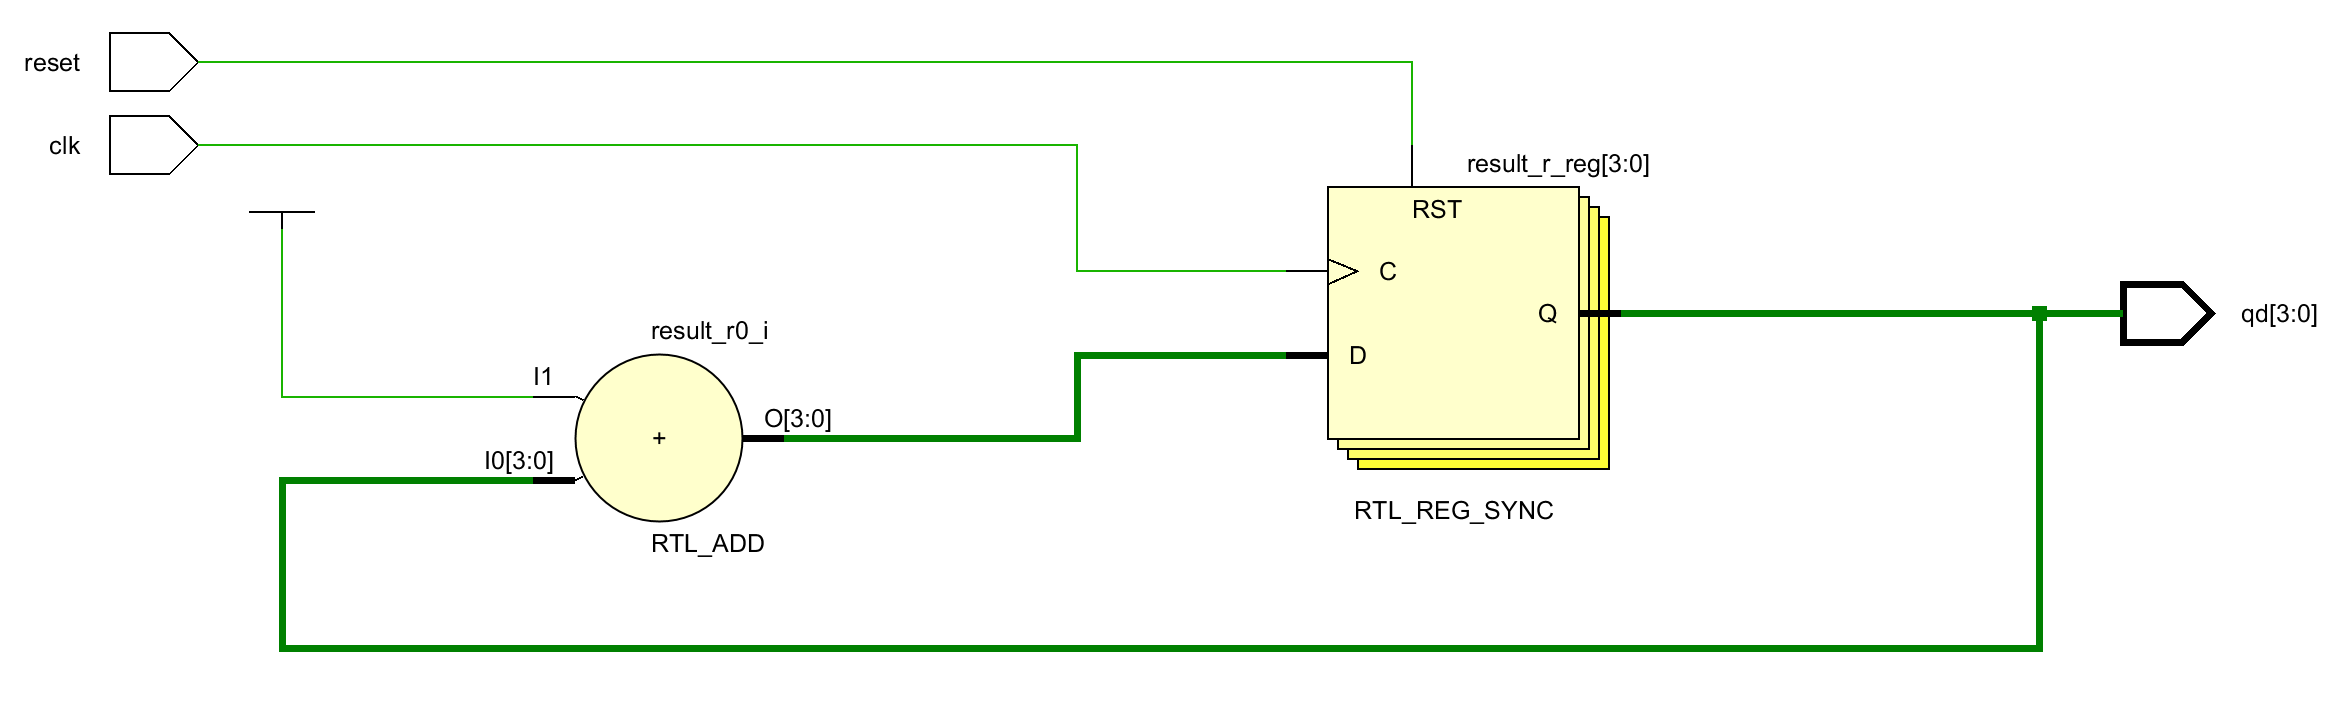
\includegraphics[width=1\linewidth]{image/counter0.png}
\end{figure}
\subsubsection{Designing a Synchronous Counter Using Verilog}
使用verilog设计4bit-同步计数器,带有同步复位输入、时钟输入和结果输出。实现中,在内部设计了一个4bit的reg用于保存当前的计数值。关于如何处理数值溢出后的绕回问题,可以考虑两种解决方案。第一种,可以在计数值=15时停止计数,直接将其赋值为0;第二种,不处理这个逻辑,因为计数值=15时已经到达了4bit能够表示的上限,再次+1会直接溢出并阶段,值自动变为0。第一种实现方法更加严谨,符合逻辑,但在电路中会导致额外的判断逻辑,导致实现中更多的门电路,而第二种方法更加适合在硬件上实现,节省资源。因此,我们选择第二种实现方案。

由于要求实现同步复位,因此在计数器递增的逻辑块的敏感列表中只需要包含时钟信号。对于同步复位而言,持续时间必须大于1个周期才能被正常识别。关于复位信号的选择,由于选择的目标器件中的D触发器都是使用高电平有效的复位信号,如果在代码中使用低电平有效的复位信号将会导致实现中多余一个反相器,造成电路浪费。因此应当根据不同的器件特性选择高或低有效的复位信号,在这里使用高电平有效的复位信号。

\subsubsection{Analysis of Design Results}
我编写了tb文件用于测试模块的正确性,起始先将复位信号拉高两个周期,再将其拉低两个周期,之后拉高12个周期,最后一直拉低。在仿真波形图中可以看出,第三周期计数器开始从0输出,输出到2时由于复位信号的影响,第4个周期开始一直保持0,12个周期后继续从0开始计数。计数达到0xf(0d16)则自动回到0,这说明我们的设计是正确的。
\begin{figure}[h]
    \centering
    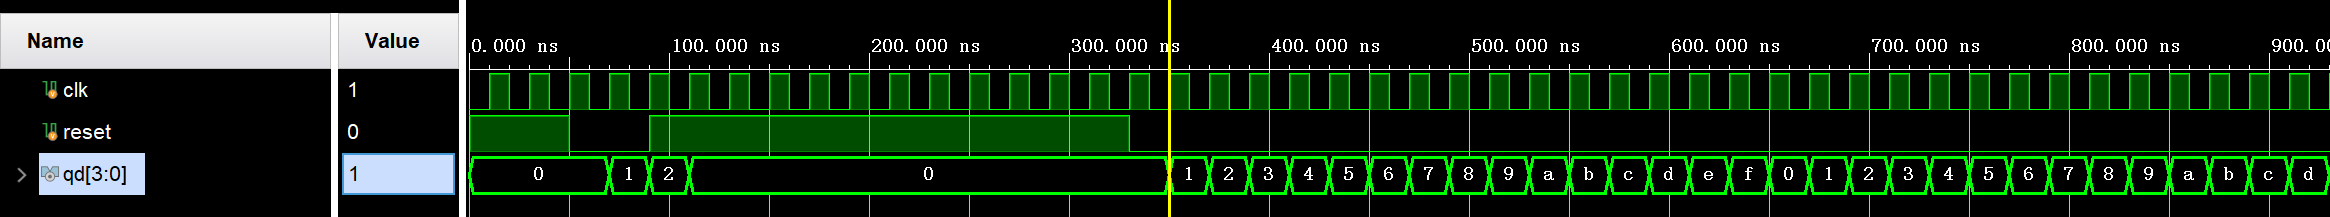
\includegraphics[width=1\linewidth]{image/problem1_result0.png}
\end{figure}
\\综合后,Vivado使用LUT完成了加法的实现,可以看到综合后的原理图如下所示:
\begin{figure}[h]
    \centering
    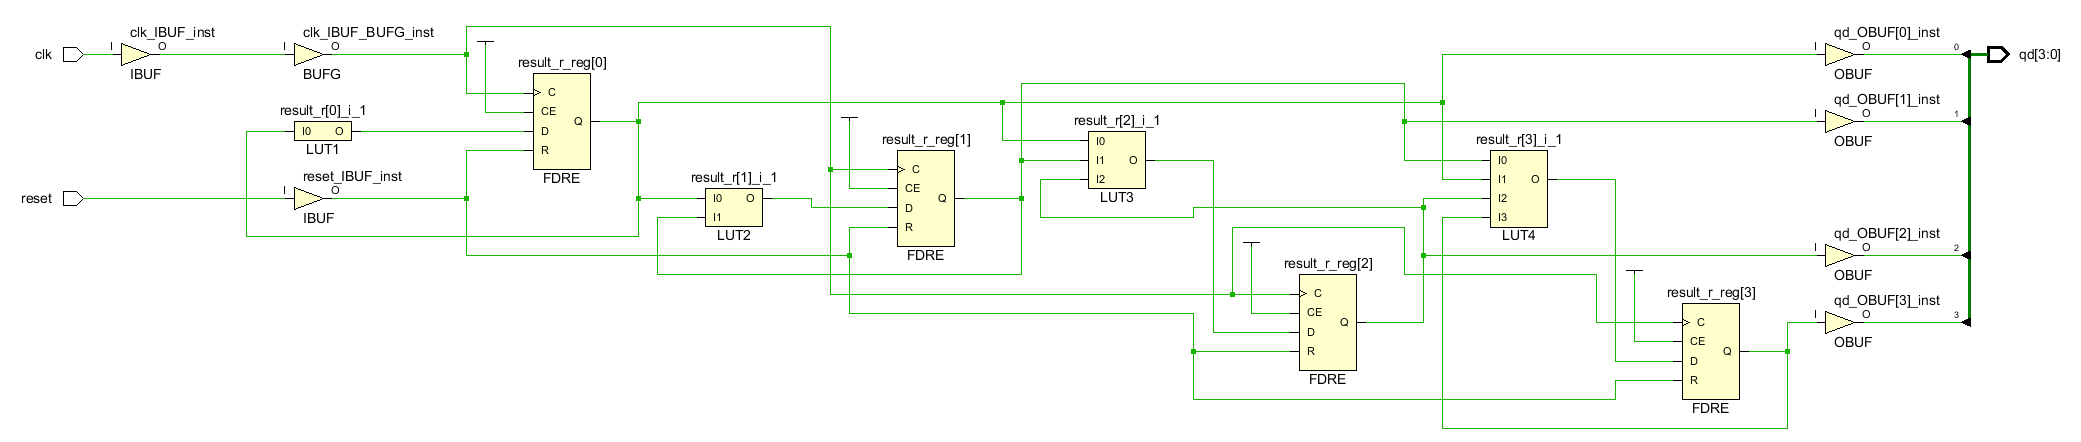
\includegraphics[width=1\linewidth]{image/counter1.png}
\end{figure}
\\在最后的设计中,使用了4个D触发器和0个反相器,这是一个可以达到的优化最佳值,因为4bit的同步计数器最少需要使用4个触发器才能实现。
\begin{figure}[h]
    \centering
    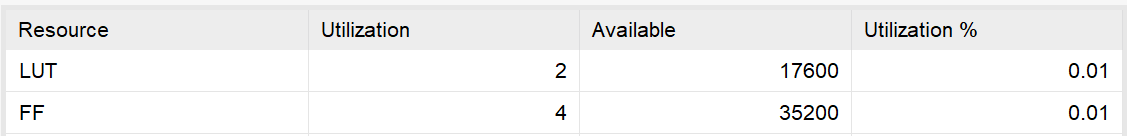
\includegraphics[width=1\linewidth]{image/problem1_result1.png}
\end{figure}
\subsection{Summary}
简单的设计中包含很多的设计哲学,能够折射出一种设计思想。虽然这是一个非常基础的模块设计,但其中的复位信号选择、自动绕回取模的实现选择等非常考验对于细节和硬件电路基础的把握。好的设计者应该充分考虑目标器件和平台的特性,并深入了解硬件描述语言如何与硬件电路产生映射关系。在这个问题的解答过程中,我也更进一步地学习了相关知识,但仍有很多不足,希望能够在不断地积累经验和尝试中进步。
\newpage
\problem{2: Knowledge Acquisition and Basic Software Tools}{20}
Perform the following steps:
\begin{enumerate}[nosep]
    \item Ask the following question to \textbf{Google Gemini} (\url{https://gemini.google.com/app}) with the \textbf{Deep Research} feature: ``Why is the COMB macro in the COMB-MCM paper better than general Compute-in-Memory macros?'' (It is a concept from one early paper of CiHlab.)
    \item Screenshot the output by Gemini.
    \item Create a public repository on your GitHub account. 
    \item Commit the screenshot picture to your repository, and push it to GitHub.
    \item Add a README to this repository (written in Markdown syntax). The content of this README should be the above picture.
\end{enumerate}

You only need to provide the URL of your GitHub repository in the answer. 
If you find it too challenging to complete all the above steps, please write down the steps you have completed and briefly explain them.

\section{The Answer to Problem 2}
我已按照要求完成全部内容,将其整理后上传到了github上。我编辑的latex源码、问题1中使用的代码也上传到了github,它的链接如下:

\url{https://github.com/Jsupermaster/Cihlab-entry-2025-JiaYutong}
\vspace{1.4in}
\newpage

\problem{3: Accelerator Design and Computer Architecture}{20}
The left figure below illustrates a roofline model of a computing hardware. Answer the following questions:
\begin{enumerate}[nosep]
    \item What does M/N mean?
    \item Now we want to deploy a DNN model to the above accelerator. During an inference, this DNN needs memory access $X$ bytes and compute operator $Y$ OPs. Under what conditions is performance limited by memory bandwidth? Under what conditions is performance limited by the size of the computing array?
    \item Given a common GPU hardware and LLM algorithm case in the figure on the right, please specify the region of the case in the roofline model and discuss the impact of memory access.
    \item One method to improve the system performance is to support the sparse matrix multiplication (SpMM) acceleration, please discuss how SpMM improve the system performance according to the roofline model and what is the overhead. (\emph{Hints}: recent GPUs support 2:4 sparsity.)
\end{enumerate}

\begin{figure}[h]
    \centering
    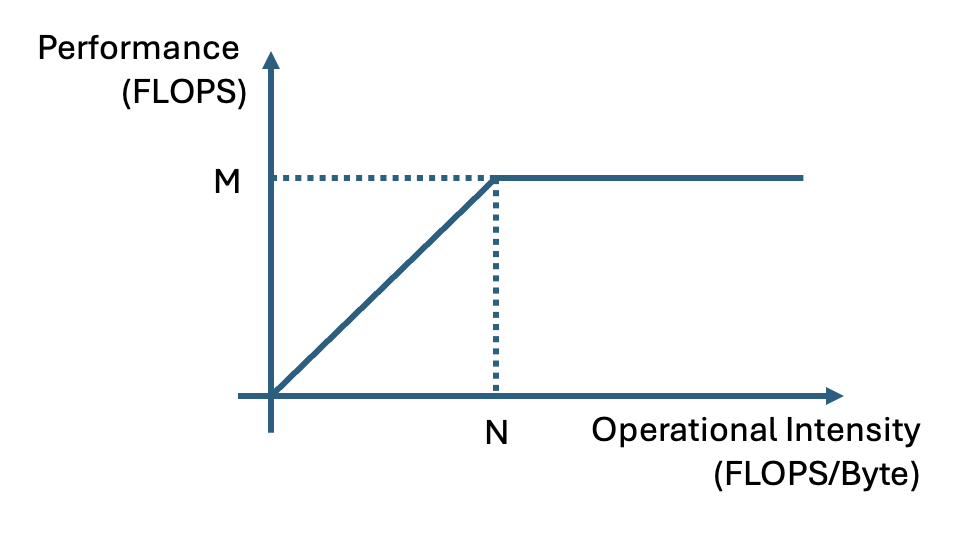
\includegraphics[width=0.48\linewidth]{image/roofline.png}
    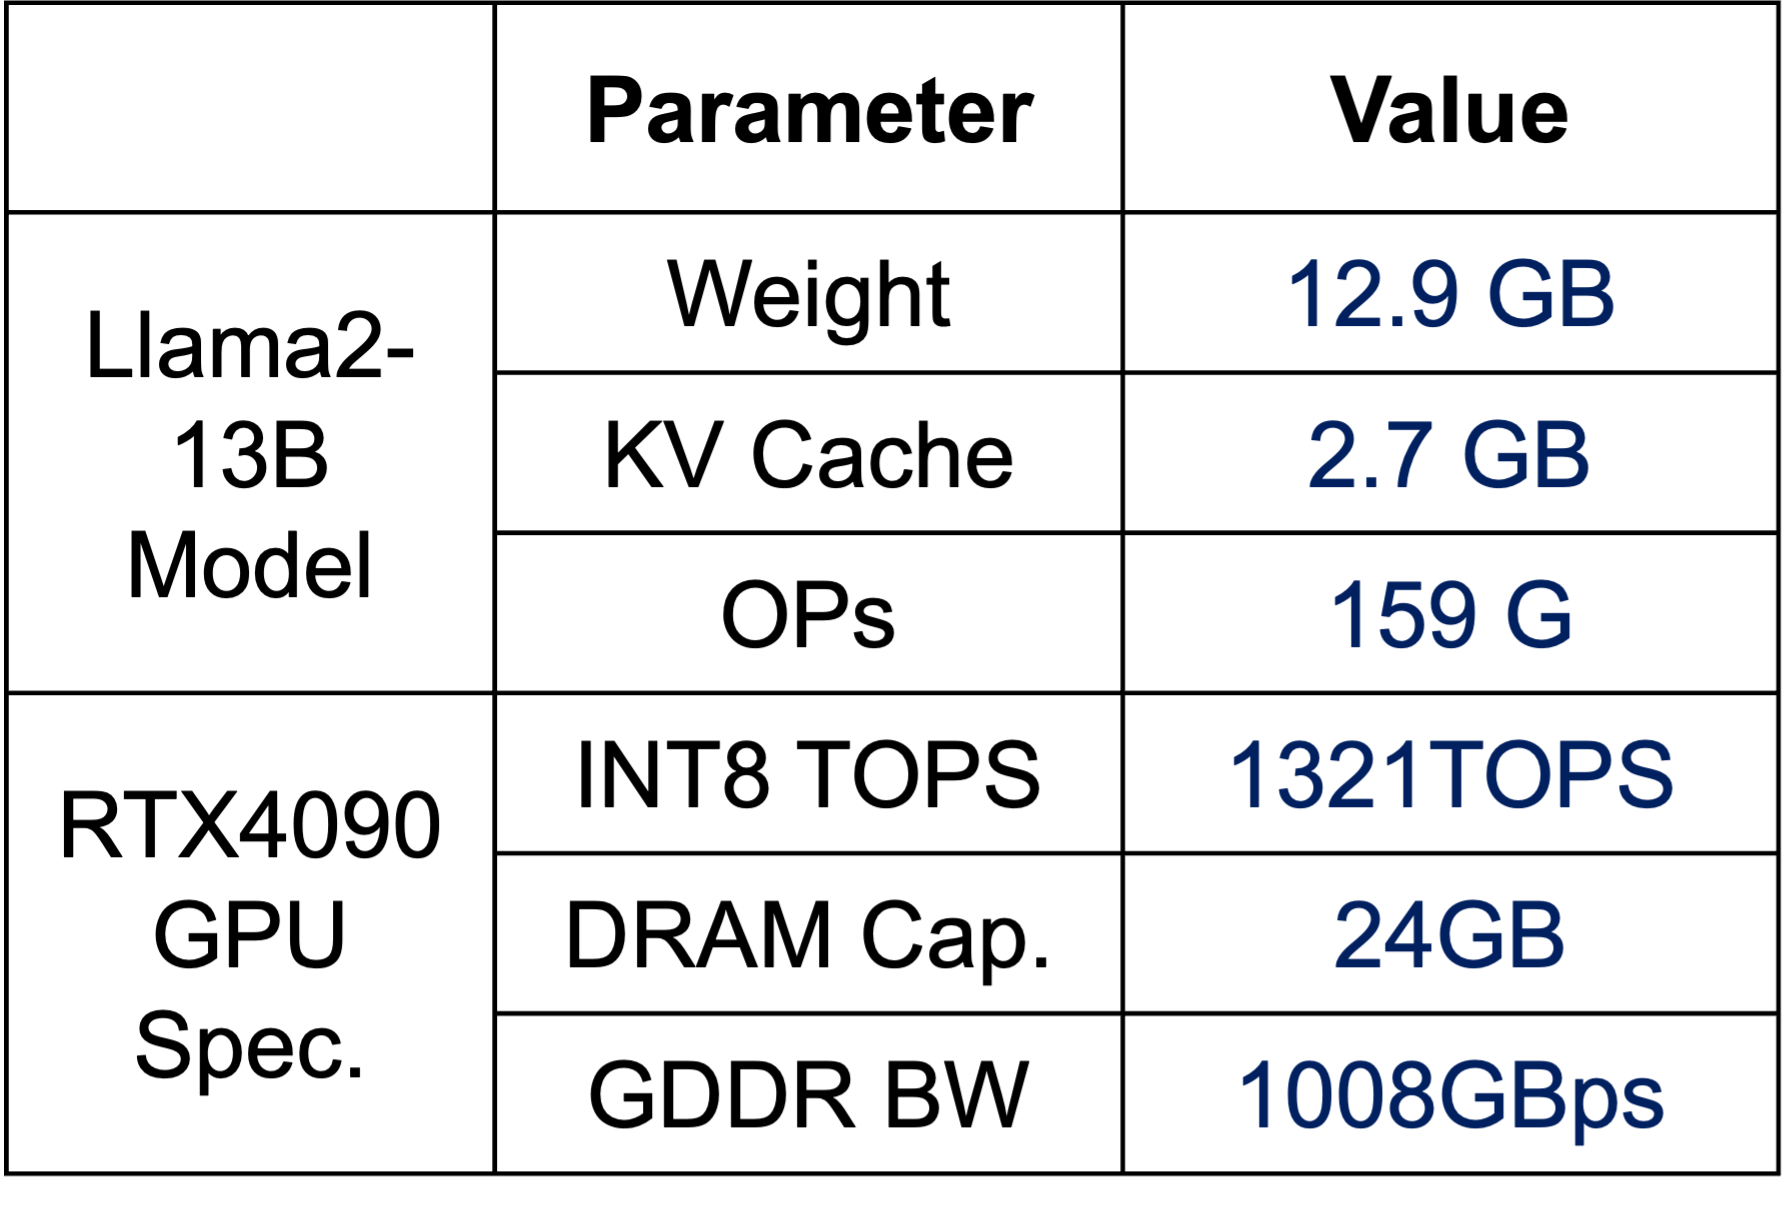
\includegraphics[width=0.36\linewidth]{image/roofline-4090.png}
    
\end{figure}
\section{The Answer to Problem 3}
\subsection{Problem Analysis}
本题目中涉及到一种常见的用于性能分析的模型——屋顶线模型。该模型常用于分析限制性能瓶颈的因素之间的关系。本题中的屋顶线模型涉及到的两个因素是FLOPS和FLOPS/Byte,说明考察的是硬件的计算能力与内存访问能力对于性能的综合影响。基于这个基本模型,有4个问题需要回答:
\begin{enumerate}[nosep]
    \item 屋顶线模型中的M和N分别代表什么含义;
    \item 在一个实际的DNN模型部署问题中,具体分析访问量和计算量将会如何受到计算瓶颈和内存访问瓶颈的限制;
    \item 基于一个实际的LLM模型数据与GPU数据分析访问量和计算量的影响;
    \item 探讨稀疏矩阵乘法是如何改善系统的性能的。
\end{enumerate}
\subsection{Background Knowledge}
解答这个问题之前,首先回顾几个关键知识点与术语。
\begin{itemize}
    \item \textbf{FLOPS:} Floating Point Operations Per Second,是用于衡量GPU或加速器等的硬件计算能力的重要参数。
    \item \textbf{FLOPs/Byte:} Floating Point Operations Per Byte,这里应该使用小写的s用于表示计算量。这是用于衡量内存与计算量之间的关系的参数,这里称为计算强度。对于计算密集的任务,计算强度较高,这时读取单Byte平均需要进行的计算量较大;而计算强度较低时,读取单Byte平均需要的计算量较少,因此需要频繁进行内存访问。
    \item \textbf{Weight:} 指模型权重的大小,反映了模型复杂度和内存需求。
    \item \textbf{KV Cache:} 键值缓存,用于自注意力机制,存储中间结果,影响推理时的内存占用。
    \item \textbf{OPs:} 模型推理所需的操作数,反映了模型所需的计算量。
    \item \textbf{INT8 TOPS:} INT8张量运算的峰值性能,适用于量化模型的推理加速。
    \item \textbf{DRAM Cap.:} 显存容量,决定能加载的模型大小和数据量。
    \item \textbf{GDDR BW:} 显存带宽,影响数据传输速度,对大规模模型和高吞吐量任务至关重要。
    \item \textbf{Quantization:} 在进行神经网络训练时,一般使用FP32的单精度浮点数;而在推理过程中,使用不同的硬件设备可能需要将原始的模型权重或输入激活以一定的方法进行量化。在GPU上运行时一般使用FP32的原始精度进行推理,但有时为了加快计算速度或减少参数存储量,也将其量化为INT8或INT4形式存储或计算。在CPU上进行推理往往需要量化为INT8精度,因为对于CPU而言浮点运算速度远低于整数运算。对于专用的硬件加速器,可以自己决定支持的数据格式;但浮点运算在更高精度的同时带来了芯片面积和功耗的显著提高。谷歌的TPU第一代仅支持INT8运算,第二代之后支持了FP16和FP32的数据格式。关于量化的详细内容在这里不进行讨论,仅讨论不同的精度带来的影响。
    
\end{itemize}
\subsection{Problem Solving}
\subsubsection{Analysis of M and N Values}
在图片所示的屋顶线模型中,M指的是硬件加速器理论上的最大计算能力,也即系统的最高性能,以FLOPS量化;而N指的是计算强度的阈值,它是计算强度的上限值,表示在这个计算平台上,单位内存交换最多用来进行多少次计算。值得注意的是,这个M和N是由硬件平台决定的,当硬件平台确定后,M和N唯一确定。不同的模型拥有不同的计算强度,因此能够利用的硬件平台算力也不同。只有当模型的计算强度高于硬件平台的最大计算强度N,才能够发挥硬件的全部性能。

屋顶线模型划分出两个瓶颈区域,当模型的计算强度小于N,则随着计算强度的增大,系统性能不断增强,这意味着此时系统性能的瓶颈是访存瓶颈;当模型的计算强度大于等于N,则随着计算强度的增大,系统性能保持最大值M不变,此时系统性能的瓶颈是计算瓶颈。计算强度较小,说明模型需要读取大量的数据,而仅需要进行小批量计算;计算强度较大,说明模型读取一批数据后需要进行大量的计算,导致平均字节计算量较高。

\subsubsection{Analysis of the Deployment of Actual DNN Models}
假设一个DNN模型需要X个字节的存储访问量,以及Y次操作。首先需要计算得出操作数/访问量,求出计算强度:
$$I = Y/X$$
当计算强度$I < N$时,说明相同的操作次数需要的访问量更高,因此,此时的系统性能受限与存储带宽。当计算强度$I > N$时,说明此时相同的访问量所需的计算量更大,已经触碰到了系统的计算性能上限M,此时的系统性能受限于计算阵列的尺寸。
\subsubsection{Analysis of LLM Model and GPU Parameters}
针对这个特定的场景,分析Llama2-13B模型和RTX4090的硬件,应该位于屋顶线模型的哪个区域。首先我们应该通过RTX4090的参数计算出屋顶线模型中的M和N,再针对Llama2模型计算出其计算强度I,通过对比判定这个系统的性能瓶颈。

在这里遇到了一些疑惑,我认为现有的数据无法满足严谨的计算需求,因此我从网络上搜集了补充的数据如下:

首先给出LLM的参数计算量公式:
\begin{align}
Parms &= L \times (Parm_{Self-Attention} + Parm_{MLP} + Parm_{LayerNorm} \times 2) \nonumber \\
      &\quad + Parm_{Embedding} + Parm_{Out-Layer} + Parm_{LayerNorm} \\
      &= L \times (12h^2 + 4h) + Vh + 2h \\
      &\approx 12Lh^2 + Vh
\end{align}

其中$L$是层数,$h$是隐藏层维度或词向量维度,$V$是词表大小。之后带入Llama2-13B的模型参数得到:
$$Parm_{Llama2-13B} = 12 \times 40 \times 5120^2 + 32000 \times 5120 = 12,746,752,000 \approx 12.75B$$

因此,Llama2-13B约有127.5亿个参数,假设每个参数按照FP32格式存储,则每个参数需要4Byte空间,共计约51GB。而为了节省存储空间和提高计算效率,模型权重通常以较低精度的格式存储,如 FP16(16 位浮点数,占用 2 个字节) 或BF16。使用FP16存储时,Llama-13B的大小理论上为:$13B \times 2 Bytes = 26GB$。
然而实际上这里给出的模型尺寸为$Weight + KV Cache = 15.6GB$,因此我们可以推断,给出的Llama2-13B模型是经过INT8量化的版本。这说明原图的屋顶线模型应该做出适当更改,以适配INT8的标准。

根据表格中RTX4090 GPU的参数,理论性能上限是1321TOPS,因此系统的计算性能上限$M = 1321TOPS$;显存带宽是1008GBps,因此所需的最小计算强度
$$N = \frac{1321TOPs/second}{1008GB/second} = 1310.516OPs/Byte$$

而Llama2-13B模型的计算强度
$$ I = \frac{OPs}{Weight + KV Cache} = \frac{159G}{15.6GB} = 10.192OPs/Byte$$

模型位于访存瓶颈区,说明此时内存瓶颈已经严重限制了模型能够利用到的硬件性能,实际只利用到约10TOPs的算力。因此可以看到,Llama2需要大量的参数用于计算,因此需要频繁地进行内存访问,而在实际部署中内存带宽不足,严重限制了硬件性能的发挥,并且距离上限非常遥远,资源利用率严重不足。
\subsubsection{Analysis of Sparse Matrix Multiplication}
在硬件上支持稀疏矩阵乘法是很好的提升系统性能的方法,想要完全分析稀疏矩阵乘法带来的性能提升,需要首先介绍稀疏矩阵的由来。

神经网络模型往往是过度参数化的,即模型可以通过剪枝去除冗余的权重。在模型的优化层面,可以按照权重单元的粒度及是否结构化,将剪枝方法的稀疏模式分为以下三类:结构化剪枝、非结构化剪枝和半结构化剪枝。其中,结构化剪枝无需专用的软硬件设计,但压缩率较低;非结构化剪枝能够获得较高的压缩率,大幅减少存储需求,但其稀疏性不具有结构化规律,会引起不规则的访存与计算,需要专用的软硬件设计;半结构化剪枝是对权重进行结构化分组,在分组内部启用非结构化稀疏模式,这样的方案具有较高的压缩率,同时引入的访存和计算模式更规则,易于在软硬件上实现,本题提到的支持2:4稀疏计算的GPU就是采用了半结构化剪枝的方法。

2:4稀疏模式要求在矩阵-矩阵乘算子中,一个输入矩阵的连续4个元素的数据组中只有2个元素非0。因此,这样的系数模式的稀疏度为50\%,这种计算模式可以通过权重剪枝产生,即将权重矩阵划分为4个元素一组的数据组,每组保留2个非0元素,并剪枝其他2个元素,激活值保持稠密格式。

如果以下图所示的算法进行2:4稀疏模式剪枝,以INT8数据格式为例,剪枝后参数量计算公式如下:
$$Parm_{purned} = Parm_{raw} \times 50\% \times (1 + 2/8) = 0.625Parm_{raw}$$
因此仅需要原来参数量的62.5\%即可完成运算。以这个结果为例,重新计算前一问的模型计算强度。
$$ I_{purned} = \frac{OPs}{(Weight + KV Cache) \times 0.625} = \frac{159G}{9.75GB} = 16.307OPs/Byte$$
约可以利用到16TOPS的算力,是剪枝前的1.6倍。
\newpage

\problem{5: Chiplet Architecture and Scablability}{20}
Given four chiplets (A, B, C, D) with limited compute and memory hardware, 
they are combined to collaborate in multiplying two large matrices:
Matrix X (divided into $X_1$, $X_2$ rows) and Matrix Y (divided into $Y_1$, $Y_2$ columns). The inter-chiplet network uses synchronous message passing with buffer constraints:

(a) Chiplet A stores $X_1$ storage, needs $Y_1$ from D to calculate $X_1Y_1$

(b) Chiplet B stores $Y_2$ storage, needs $X_1$ from A to calculate $X_1Y_2$

(c) Chiplet C stores $X_2$ storage, needs $Y_1$ from B to calculate $X_2Y_1$

(d) Chiplet D stores $Y_1$ storage, needs $Y_2$ from C to calculate $X_2Y_2$

(e) Each chiplet only has two data buffer slots for die-to-die interface, and the inter-chiplet communication latency is 500ns $\pm$ 100ns. The buffer allocation timeout is 2µs, and die-to-die bandwidth is 32GBps/buffer-slot.
Questions:

(1) Draw the time diagram for a complete matrix multiplication $X\cdot Y$. (\emph{Hints}: A→B→C→D→A)

(2) Calculate the minimum buffer duration for Chiplet C, when receiving $Y_1$ (230MB) from Chiplet B, forwarding $X_2$ (210MB) to Chiplet D, and processing local  $X_2Y_1$ (1.5µs) simultaneously. Assuming that buffer multiplexing and system control overhead are (15\%).

(3) Discuss the potential deadlock probability among these chiplets if multiple requests are involved. 

\section{The Answer to Problem 5}
\subsection{Problem Analysis}
本题中涉及到芯粒技术和多芯片信息传输问题。题目中的表述可能存在一些笔误,为了便于描述,我按照我的理解和逻辑,重新整理已知条件:
\begin{figure}[h]
    \centering
    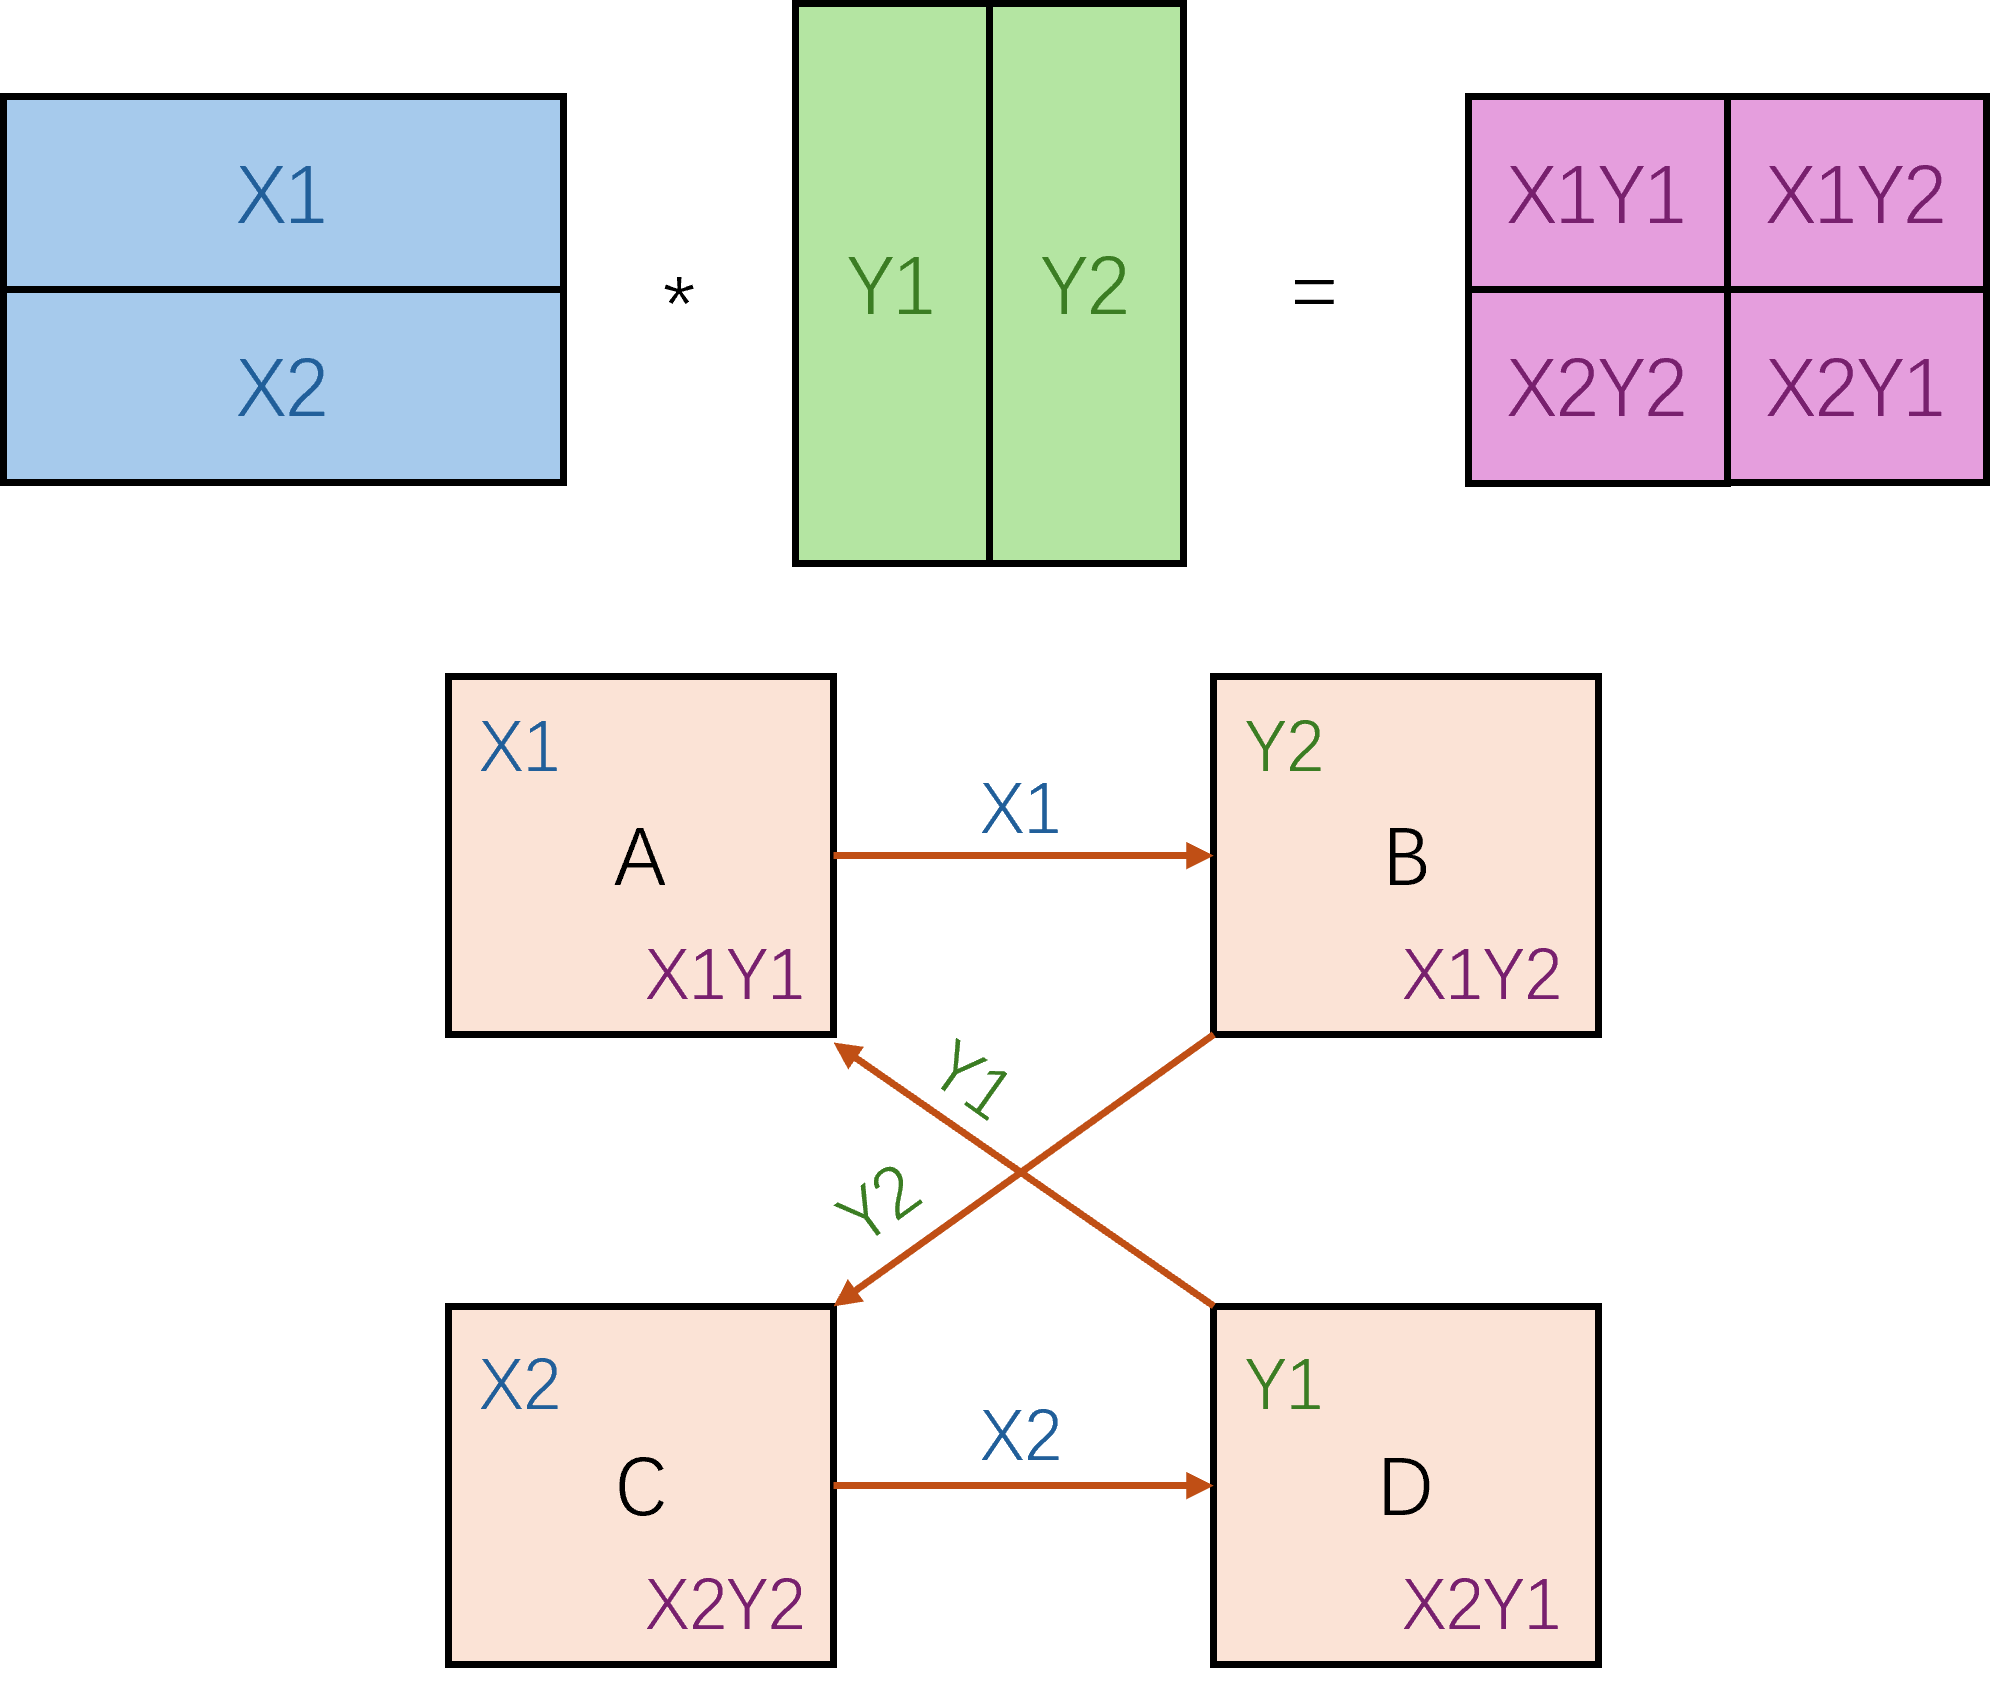
\includegraphics[width=0.7\linewidth]{image/problem5_1.png}
\end{figure}
\begin{itemize}
    \item 现在有A,B,C,D四个芯粒,每个芯粒的计算资源和存储空间有限;
    \item 需要进行的计算是$X \cdot Y$,其中$X$被按行分成$X_1$和$X_2$,$Y$被按列分成$Y_1$和$Y_2$;
    \item 芯粒之间使用同步信息传输,即需要满足握手机制;
    \item A存储的是$X_1$的数据,需要从D中获得$Y_1$数据,用于计算$X_1Y_1$;
    \item B存储的是$Y_2$的数据,需要从A中获得$X_1$数据,用于计算$X_1Y_2$;
    \item C存储的是$X_2$的数据,需要从B中获得$Y_2$数据,用于计算$X_2Y_2$;
    \item D存储的是$Y_1$的数据,需要从C中获得$X_2$数据,用于计算$X_2Y_1$;
    \item 每个芯粒拥有2个数据缓冲区,芯片间通信延时是500ns$\pm$100ns,数据缓冲区超时自动释放时间是2µs,芯片间的通信带宽是每个数据缓冲区32GBps。
\end{itemize}
根据以上的已知条件,需要回答下列三个问题:
\begin{enumerate}[nosep]
    \item 绘制矩阵乘法$X \cdot Y$的时序图;
    \item 当C从B接收到$Y_2$(230MB),并把$X_2$(210MB)发送到芯片D,同时计算本地的$X_2Y_2$(1.5µs),计算C的数据缓冲区最小缓冲时间,假设缓冲区复用和系统控制的开销比是15\%;
    \item 探讨在多个请求并发时,这些芯粒之间潜在的死锁风险可能性。
\end{enumerate}
\subsection{Background Knowledge}
解答这个问题之前,首先回顾几个关键知识点与术语。
\begin{itemize}
    \item \textbf{Chiplets:} Chiplet是一类具有特定功能的晶片(die,也称为裸片)。这些晶片,可以是使用不同工艺节点制造,甚至是不同的半导体公司制造,可以由不同的供应商提供,可以采用不同材质(硅、砷化镣、碳化硅等)。多个Chiplet通过特定设计架构和先进封装技术,集成在一起实现完整功能,能突破目前单一芯片设计的瓶颈。和单一芯片设计模式相比,Chiplet设计模式具有更短的设计周期、更低的设计成本、更高的良率等突出优点。
    \item \textbf{Handshaking Mechanism:} 握手机制是通信过程中常用的一种请求-接收确认方法。一般通信双方都具有准备接收信号、数据收发端口和信息交换端口。由一方发起发送请求,另一方相应并返回一个值,发起方确认值后正式建立通信。
    
\end{itemize}
\subsection{Problem Solving}
\subsubsection{Drawing of Sequence Diagrams}
每个芯粒都包含两个数据缓冲区,而根据分析,每个芯粒都需要从另一个芯粒接收数据,并把自己存储的内容发送给另一个芯粒。因此,理论上芯粒可以同时完成发送数据、接收数据和计算数据的任务。但由于使用同步信息传输,因此需要由一个芯粒率先发起请求,再按照顺序完成数据发送过程。一个可能的发送-接收过程是这样的:
\\A请求向B发送$X_1$ --> B请求向C发送$Y_2$ --> C请求向D发送$X_2$ --> D请求向A发送$Y_1$ 
\begin{figure}[h]
    \centering
    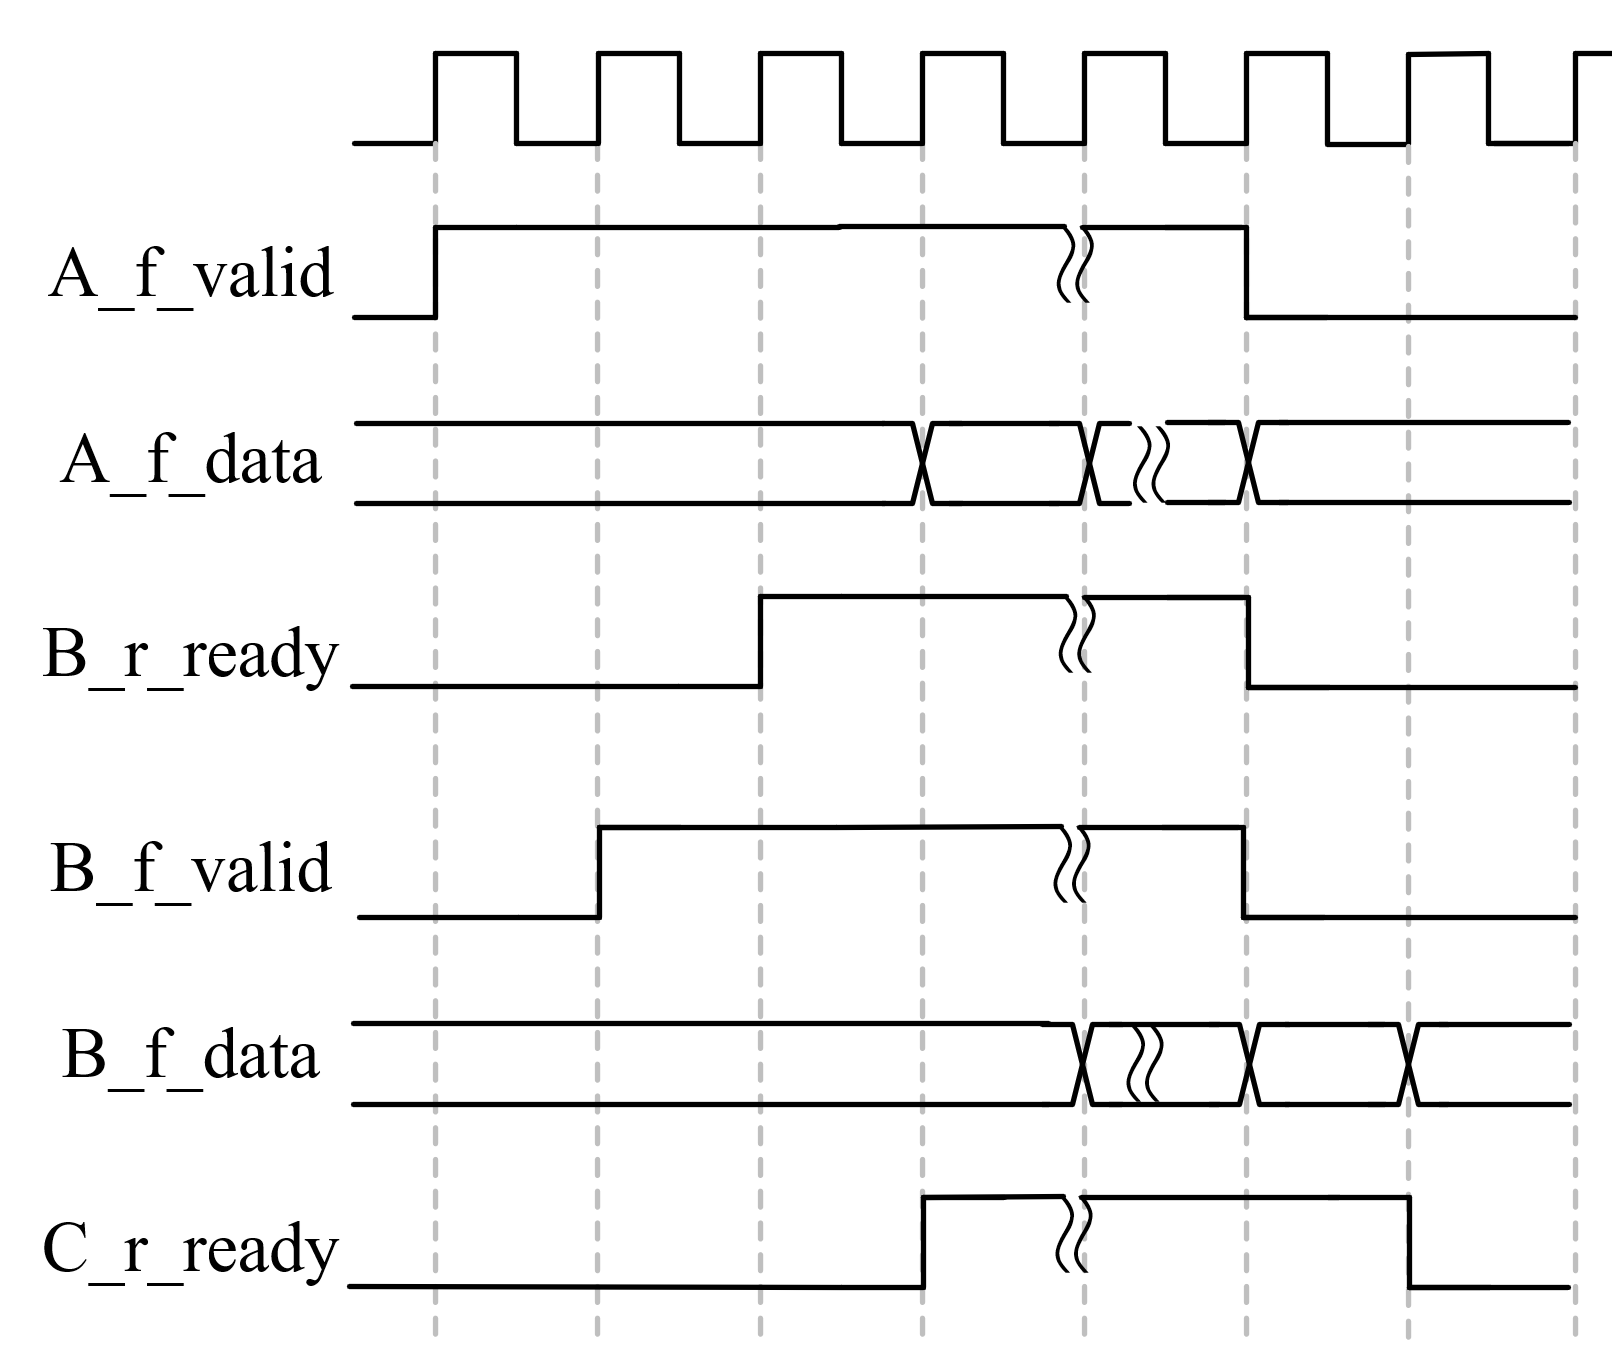
\includegraphics[width=0.7\linewidth]{image/time.png}
\end{figure}

我们假设每个芯粒拥有两组数据发送-接收端口,均可以实现双向握手。假设每个芯粒包含的握手信号都是如下几种:
\begin{itemize}
    \item \textbf{r\_ready:} output,准备接收信号
    \item \textbf{r\_valid:} input,接收有效信号
    \item \textbf{r\_data:} input,接收数据
    \item \textbf{f\_ready:} input,准备发送信号
    \item \textbf{f\_valid:} output,发送有效信号
    \item \textbf{f\_data:} output,发送数据
\end{itemize}
为了便于时序图描述,以A发送,B接收为例,A一侧的f\_ready就是与B一侧的r\_ready,因此时序图中统一使用r\_ready表示。
发送的一般流程是,接收方一直处于ready状态,发送方开始拉高valid信号。同时开始数据传输,期间ready和valid信号一直拉高,若干个周期后数据传输结束,valid信号拉低。

\subsubsection{Analysis of Buffer Time for C}
C同时需要发送数据和接收数据,接收数据所需的时间是:
$$time_r = \frac{Size_{Y_2}}{Bandwidth} + time_{delay} = \frac{230MB}{32GB/s} + 500ns \approx 7.188ms$$

发送数据所需的时间是:
$$time_f = \frac{Size_{X_2}}{Bandwidth} + time_{delay} = \frac{210MB}{32GB/s} + 500ns \approx 6.563ms$$

计算所需的时间是:
$$time_{cal} = 1.5 µs$$

由于同时进行计算和缓冲区复用控制,造成用时增加15\%,而缓冲区被占用的最短时间应该是发送、接收和计算三者中较长的一个:
$$time_{buffer} = max(time_r, time_f, time_{cal}) \times 115\% = 8.2662ms $$

在这里存在几个疑惑。第一,除了两个数据缓冲区,每个chiplet内部是否存在可用于存储数据的DRAM或SRAM,因为在计算过程中仍然需要存储空间。也就是说,每个chiplet至少包含三大部分存储空间,两个数据缓冲区空间和一个内部的计算缓存空间。假设有这样的空间,那么计算过程可以和数据发送完全分离,但是会导致数据额外存储一份,浪费了资源。假设没有这样的空间,那么数据缓冲区应该支持双端口读出,使得内部的计算单元和发送模块可以同时读取数据缓冲区。如果不支持双端口读取,那么只能等待内部计算结束后再发送数据,但这样导致浪费了一定的时间,尽管计算时间与数据传输时间相比是很短的。

另一个疑惑是,数据缓冲区存在2µs的超时限制,这个限制是否是针对所有的时间而言,比如发送、接收的操作都不能占用数据缓冲区超过2µs,还是这个限制仅存在于握手期间,只有当请求在2µs内未被相应,才会被中止,而正常的数据发送、接收不受限制?

综合上述,以上的分析建立在计算与发送/接收可以完全同步的情况下,且假设数据缓冲区超时限制仅存在于握手期间,数据传输期间不受到这个限制。

\subsection{The Possibility of Deadlock and The Associated Risks}
如果严格按照时序流程进行,则不会出现死锁问题。但如果处于多个请求并发,在这样的情况下可能存在死锁风险。死锁发生的四个必要条件是:互斥、持有并等待、不可抢占和循环等待。有可能出现以下死锁情况:
\begin{itemize}
    \item 循环依赖死锁:多个芯片之间形成循环等待对方释放资源的情况,例如A等D,D等C,C等B,B等A。
    \item 资源竞争死锁:多个传输任务竞争有限的缓冲槽,导致彼此都无法完成传输,进而无法释放资源。
    \item 重传导致的死锁:超时重传过程中,多次重试占用资源,无法完成传输,导致其他任务无法获得资源。
    \item 流水线阶段阻塞:流水线中某一阶段因数据不完整而停滞,导致前后阶段无法推进,形成阻塞。
\end{itemize}

\problem{7: Presentation Skills}{25}
Prepare a PowerPoint presentation (approximately 10 slides) introducing one of the following: a) a research project you have worked on, b) a competition you participated in, c) a course design you have completed. 

The slides should be structured as follows: a) Background, b) Key Challenges, or c) Innovative Solution, d) Experimental Setup and Results, e) Your Contribution to the work. 

It is recommended that you use English for the presentation. Focus on presenting the depth of your work rather than its breadth. Once completed, please attach the presentation PDF along with your answer sheet in the email.

\section{The Answer to Problem 7}
我的英语汇报PPT已经转换为PDF附在邮件中,请老师查看。

[摘要]我在10页PPT中简要介绍了我的一项科研经历,内容是关于BNN的网络设计和硬件加速器设计。在这段研究工作中,我主要负责和参与了:论文整理与创新点归纳总结,结合我在CPU设计和体系结构中学习的保留站结构,提出了引入乱序调度的创新思路、部分模块代码编写、模块测试、论文撰写等。

\section{References}
本解答中使用或参考的资料如下:
\begin{enumerate}[nosep]
    \item 数字电路与逻辑设计,林红等,清华大学出版社
    \item 搭建你的数字积木--数字电路与逻辑设计(Verilog HDL\&Vivado版),汤勇明等,清华大学出版社
    \item 数字电子技术基础(第六版),阎石等,高等教育出版社
    \item \url{https://blog.csdn.net/q774318039a/article/details/88828873}
    \item Vivado Design Suite 7 Series FPGA and Zynq 7000 SoC Libraries Guide (UG953)
    \item \url{https://zhuanlan.zhihu.com/p/34204282}
    \item \url{https://www.aisharenet.com/damoxingcanshuliangba/}
    \item \url{https://blog.csdn.net/spx1164376416/article/details/124624351}
    \item \url{http://www.ictest8.com/a/technology/semi/2023/11/Chiplet.html}
    \item \url{https://zhuanlan.zhihu.com/p/34204282}
    \item \url{https://zhuanlan.zhihu.com/p/677057296}
\end{enumerate}
本解答中的部分内容参考了LLM Chatbots的回答:

1.锁存器和触发器有什么区别和联系?

Latches and flip-Flops: Key Differences and Connections  
Both latches and flip-flops (FFs) are fundamental 1-bit memory elements in digital circuits, but they differ in operation, timing, and usage.  
1. Basic Definitions  
A. Latch  
- Level-triggered: Changes output when the enable signal (E) is active (high/low).  
- Example: A D-latch transparently passes input D to output Q while E=1 and holds when E=0.  
- No clock edge dependency: Controlled by an enable signal instead of a clock.  
- Common types: SR latch, D latch, Transparent latch  
B. Flip-Flop (FF)  
- Edge-triggered: Updates output only at a clock edge (rising/falling).  
- Example: A D flip-flop captures D at the clock edge and holds it until the next edge.  
- Clock-dependent: Requires a clock (CLK) signal.  
- Common types: D flip-flop, JK flip-flop, T flip-flop  
2. Key Differences  
Feature          Latch                          Flip-Flop  
Trigger Method   Level-sensitive (E=1/E=0)      Edge-sensitive (clock edge)  
Clock Signal     No clock (uses enable)         Requires clock (CLK)  
Output Update    Transparent when enabled       Sampled only at clock edge  
Glitch Immunity  Low (susceptible to glitches)  High (stable at edges)  
Timing Analysis  Harder (race conditions)       Easier (predictable timing)  
Usage            Asynchronous designs           Synchronous designs  
3. Connections Between Them  
- Both store 1-bit data  
- Can be converted: Two latches form a flip-flop  
- Verilog Implementation:  
  Latches: Generated with incomplete if/case  
  Flip-flops: Explicitly coded with always @(posedge clk)  
4. Why Flip-Flops Are Preferred?  
- Better for synchronous design  
- More stable timing control  
- Better supported by EDA tools  
5. When to Use Latches?  
- Asynchronous interfaces  
- Low-power circuits  
- Custom storage needs  
Example D Latch in Verilog:  
module d\_latch (input D, E, output reg Q);  
always @(*) begin if (E) Q = D; end  
endmodule  
Conclusion  
- Latches: Simpler but riskier  
- Flip-Flops: Robust and preferred for synchronous designs  
Design Tip: Avoid unintentional latches in combinational logic by covering all if/case conditions.

\textbf{My Contuibutions:} 我总结并整理了回答,将其结合课本上的内容和查询到的资料,重新梳理在上面的回答中。

2.A brief introduction to the grip mechanism.

**Handshake Mechanism**  
A handshake mechanism is a foundational process in communication or interaction where two parties establish a connection, confirm status, or synchronize information. Its core purpose is to ensure mutual agreement before formal data transmission, preventing errors or miscommunication.  

**Key Functions**:  
1. **Connection Verification**: Validate communication channel availability (e.g., TCP three-way handshake via client-server signal exchanges).  
2. **Parameter Negotiation**: Agree on encryption algorithms (e.g., SSL/TLS handshake), data transfer rates, etc.  
3. **Authentication**: Used in security scenarios, such as key exchange during Wi-Fi connections.  
4. **State Synchronization**: Ensure both parties are ready (e.g., Bluetooth device pairing initialization).  

**Typical Steps**:  
- **Request**: One party initiates a connection request (e.g., SYN packet).  
- **Response**: The other party acknowledges and returns parameters (e.g., SYN-ACK).  
- **Final Confirmation**: The initiator confirms parameters to formalize the connection (e.g., ACK).  

**Applications**:  
- Network protocols: TCP three-way handshake, TLS encryption handshake.  
- Hardware interactions: USB device enumeration with a host.  
- Security authentication: Handshake verification before digital certificate exchange.  

This mechanism ensures reliability in complex communication through simple interactive steps, serving as a fundamental safeguard for digital interactions.

\textbf{My Contuibutions:} 我总结并整理了回答,整合了我搜集的资料,将其简洁地整理在回答中。


\end{document}
